\chapter{Road Mapping}
\section{Overview}
\subsection{Context}
Objective of year 4 is to bring together all your knowledge from your undergraduate courses and see how it can be applied to real practical problems. Graduate level courses put the emphasis on the student to find and read around the material.
\begin{itemize}
    \item First, we will explore what we mean by the words ``extreme pressure'', ``extreme chemistry'' and ``extreme temperature''
          \begin{itemize}
              \item \dots by looking at a number of examples
          \end{itemize}
    \item Structure of the courses - the role of the professor and your role
    \item Formalisation of these definitions and classifications
    \item How does industry deal with these problems
\end{itemize}
\subsection{Course assessment}
\textbf{Assessments}
\begin{enumerate}
    \item Coursework (30\%) - January
    \item Group Project (40\%) - end of March
    \item Laboratory class (30\%) - February
\end{enumerate}
1, 2, 3 will cover the three themes of pressure, temperature and chemistry.
\begin{table}[htbp]
    \centering
    \begin{tabular}{@{}llll@{}}
        \toprule
                      & \textbf{2018-2019}    & \textbf{2019-2020}            & \textbf{2020-2021}            \\
        \midrule
        Exam          & Extreme Pressure      & Extreme Temperature           & CW Extreme Temperature        \\
        Group Project & Extreme Temperature   & Extreme Pressure              & Extreme Pressure              \\
        Laboratory    & Corrosion (chemistry) & Extreme chemistry (corrosion) & Extreme chemistry (corrosion) \\
        \bottomrule
    \end{tabular}
    \caption{Table to show themes of assessments in previous years.}
\end{table}
\subsection{Group project - extreme pressure 2019 / 2020}
You must choose which problem you are interested in and we will organise you into groups. We will have a fortnightly session to discuss through the term and give you help. We will be running training sessions so that everyone has a chance to learn a bit about CFD. Need to raise the game from last year - tended to have a late start.
\subsection{Course structure}
4 teaching blocks:
\subsubsection{Block 1}
Lectures 1-4:
\begin{itemize}
    \item Setting the scene, framework and terminology
    \item Investigative tools used to solve hard problems
    \item Key concepts for molecular scales (chemistry and materials)
    \item Key concepts for continuum scales (fluid mechanics, solid mechanics and structures)
\end{itemize}
\subsubsection{Block 2}
Lectures 5-8: Extreme Pressure.
\begin{itemize}
    \item Static cases
          \begin{enumerate}
              \item High pressure: bottom of the ocean, pressure vessels
              \item Low pressure: space, cavitation
          \end{enumerate}
    \item Unsteady cases
          \begin{enumerate}
              \item High pressure: gas flows, AIV, explosions (nuclear), liquid flows, VIV, TIV
              \item Low pressure: cavitation
          \end{enumerate}
\end{itemize}
\subsubsection{Block 3}
Lecture 9-12: Extreme Chemistry.
\begin{itemize}
    \item Slow chemistry
          \begin{enumerate}
              \item Corrosion
          \end{enumerate}
    \item Fast chemistry
          \begin{enumerate}
              \item Fuel cells
              \item Combustion
          \end{enumerate}
    \item Application section: manufacturing, design and testing
\end{itemize}
\subsubsection{Block 4}
Lecture 13-16: Extreme Temperature.
\begin{itemize}
    \item Static cases
          \begin{enumerate}
              \item High temperature: fire, manufacturing, coatings
              \item Low temperature: arctic, LNG transport
          \end{enumerate}
    \item Unsteady cases
          \begin{enumerate}
              \item Thermal shocks
          \end{enumerate}
\end{itemize}
\section{Engineering in extreme environments}
What do we mean by these words?
\begin{quoting}
    The phrase "engineering in extreme environments" relates to the study, design, and implementation of engineering solutions that can withstand and function optimally under extremely harsh or atypical conditions. These conditions are characterized by extreme pressure, extreme temperature, and extreme chemical environments, all of which present unique challenges that can significantly affect the performance and durability of materials and systems.

    Specifically:

    Extreme Pressure: Engineering in high-pressure environments often involves deep-sea, subterranean or aerospace applications, where the equipment is subjected to extraordinary pressures. This requires an in-depth understanding of material properties and structural integrity under such conditions, including factors like compression, shear stress, and deformation.

    Extreme Temperature: This refers to the ability to design and implement engineering solutions in environments with very high or very low temperatures. This might include deep-sea vents, cryogenic systems, combustion engines, or spacecraft re-entry systems. The challenges here primarily relate to thermal stress, material expansion/contraction, and maintaining operational efficiency under these temperature ranges.

    Extreme Chemistry: Engineering in extreme chemical environments requires developing materials and systems that can resist highly corrosive or reactive environments, which can include certain industrial processes, chemical plants, or hostile extraterrestrial environments. An understanding of material science, including the resistance of different materials to corrosion, oxidation, and other chemical reactions, is crucial.

    This aspect of mechanical engineering seeks to unite the foundational knowledge of mechanical engineering — such as fluid mechanics, thermodynamics, materials science, and structural analysis — with a deeper understanding of how these principles apply under extreme conditions. It typically involves rigorous testing and modelling, the use of advanced materials and coatings, and innovative design principles to ensure safety, efficiency, and longevity of engineering systems under extreme environments.

    (ChatGPT-4 2023-07-03)
\end{quoting}
\subsection{Engineering}
Engineering - a branch of science and technology concerned with the design, building, and use of engines, machines, and structures.

Focussed on the discrete elements or components that sit in an environment. We will refer to a structure throughout the course, through what we really mean is anything (engine, blade, casing, tool, system, person).
\subsection{Classification of environment}
Environment - this is just the surroundings in which an objects sits or is exposed to. There are two types of environments:
\begin{enumerate}
    \item Natural
    \item Man-made
\end{enumerate}
There has to be a physical way to communicate between the environment and the engineering structure which is usually through a surface.
\subsection{Classification of interactions}
\begin{itemize}
    \item Internal or closed problems e.g. pipe flow, IC engine
    \item Open problems e.g. fire outside, atmospheric
          \begin{itemize}
              \item Open problems represent challenges in terms of boundary conditions
          \end{itemize}
\end{itemize}
\subsubsection{Types of interactions}
\begin{itemize}
    \item Interactions are with the interfaces. What processes act on an interface?
    \item Solid surface - affected by:
          \begin{itemize}
              \item normal / tangential forces / pressure / viscous forces (high / low pressure)
          \end{itemize}
    \item Thermal effects (heating / cooling)
    \item Chemical effects (burning, corrosion)
    \item Structural changes due to forces / loading
    \item Fatigue
\end{itemize}
\subsubsection{Interfacial processes}
\begin{itemize}
    \item Temperature
    \item Stresses - solid and fluid forces
    \item Chemistry
\end{itemize}
\subsection{Classification of extremes}
Extreme has quite a few interpretations. Extreme may be something that is an outlier. The definition that we will work around is based on two types:
\begin{enumerate}
    \item based on magnitude (of a scalar or vector)
    \item how it is spread and varies spatially or temporally
\end{enumerate}
We try to tackle these broad questions using regime diagrams (Figures \ref{regimeDiagram1}, \ref{regimeDiagram2}, \ref{regimeDiagram3}).
\begin{figure}[htbp]
    \centering
    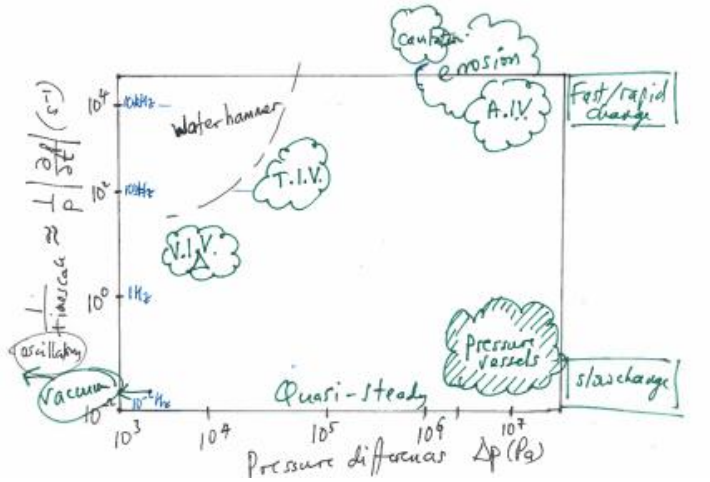
\includegraphics[width = 0.8\textwidth]{./img/figure78.png}
    \caption{Regime diagram to show different pressure environments.}
    \label{regimeDiagram1}
\end{figure}
\begin{figure}[htbp]
    \centering
    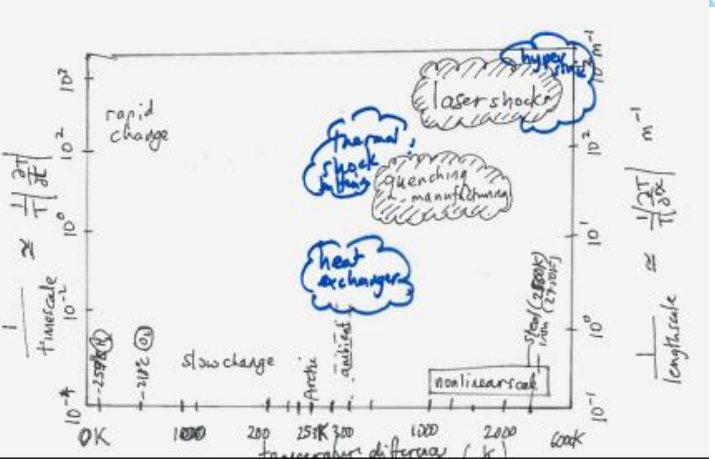
\includegraphics[width = 0.8\textwidth]{./img/figure79.png}
    \caption{Regime diagram to show different temperature environments.}
    \label{regimeDiagram2}
\end{figure}
\begin{figure}[htbp]
    \centering
    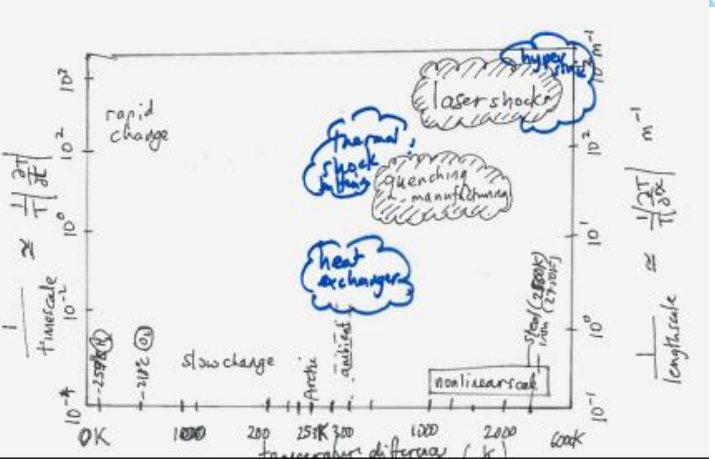
\includegraphics[width = 0.8\textwidth]{./img/figure79.png}
    \caption{Regime diagram to show different chemical environments.}
    \label{regimeDiagram3}
\end{figure}
\section{Extreme natural environments}
\begin{table}[htbp]
    \centering
    \begin{tabular}{@{}ll@{}}
        \toprule
        \textbf{Under extreme} & \textbf{Examples}            \\
        \midrule
        Pressure               & Tsunami, earthquakes, storms \\
        Temperature            & Fires, arctic                \\
        Chemistry              & Corrosion, biofouling        \\
        \bottomrule
    \end{tabular}
    \caption{Table to show example naturally extreme environments.}
\end{table}
\subsubsection{Challenges in extreme natural environments}
Main challenges are:
\begin{enumerate}
    \item Living in these external environments
    \item Working in these external environments
\end{enumerate}
\subsection{Extreme pressure}
\subsubsection{Example: deep water (high pressure)}
\begin{quoting}
    Deep underwater environments, such as those over 2000 meters below sea level, experience extreme hydrostatic pressure. This pressure can pose severe challenges to structures, equipment, and human life. For instance, habitats in deep oceans and lakes must be designed to withstand these pressures. A case in point is the Deepwater Horizon oil drilling rig, which suffered a catastrophic failure in 2010. The disaster was partly attributed to a mismanagement of high-pressure conditions approximately 1000 meters below sea level, highlighting the critical role that pressure management plays in these environments.

    (ChatGPT-4 2023-07-03)
\end{quoting}
\subsubsection{Example: hurricanes (high pressure and gustiness)}
\begin{quoting}
    Hurricanes present a convergence of extreme conditions. The high wind pressure and gustiness can lead to severe infrastructural damage. These natural disasters are formed from a convergence of tropical thunderstorms, leading to an area of low pressure with high winds blowing into the area. Over 2000 deaths have occurred due to hurricanes in the US since 2005. The combination of high pressure, high winds, and water hazards like storm surges and flooding make them a multifaceted challenge.

    (ChatGPT-4 2023-07-03)
\end{quoting}
\subsubsection{Example: earthquakes (high solid mechanical pressure)}
\begin{quoting}
    Earthquakes generate extreme solid mechanical pressures resulting from seismic activity. The vibration of the ground due to surface waves can lead to the failure and collapse of structures, making it a significant challenge for civil and structural engineers to design buildings that can withstand these forces. On average, earthquakes result in around 10,000 fatalities per year, indicating the severity of their impact and the importance of engineering designs that consider seismic activity.

    (ChatGPT-4 2023-07-03)
\end{quoting}
\subsubsection{Example: tsunami (high fluid pressure)}
\begin{quoting}
    Tsunamis represent a high-impact hazard that involves enormous fluid pressures. Generated by underwater seismic activity, landslides, or volcanic eruptions, tsunamis can travel across ocean basins and cause massive destruction when they make landfall. A devastating example of this is the 2004 Indian Ocean tsunami, which resulted in the deaths of over 230,000 people. Designing for tsunami resistance, especially in coastal areas, involves understanding and accounting for these extreme fluid pressures in order to protect structures and lives.

    (ChatGPT-4 2023-07-03)
\end{quoting}